%UCE-2: Monitorizza evento

\begin{figure}
\centering
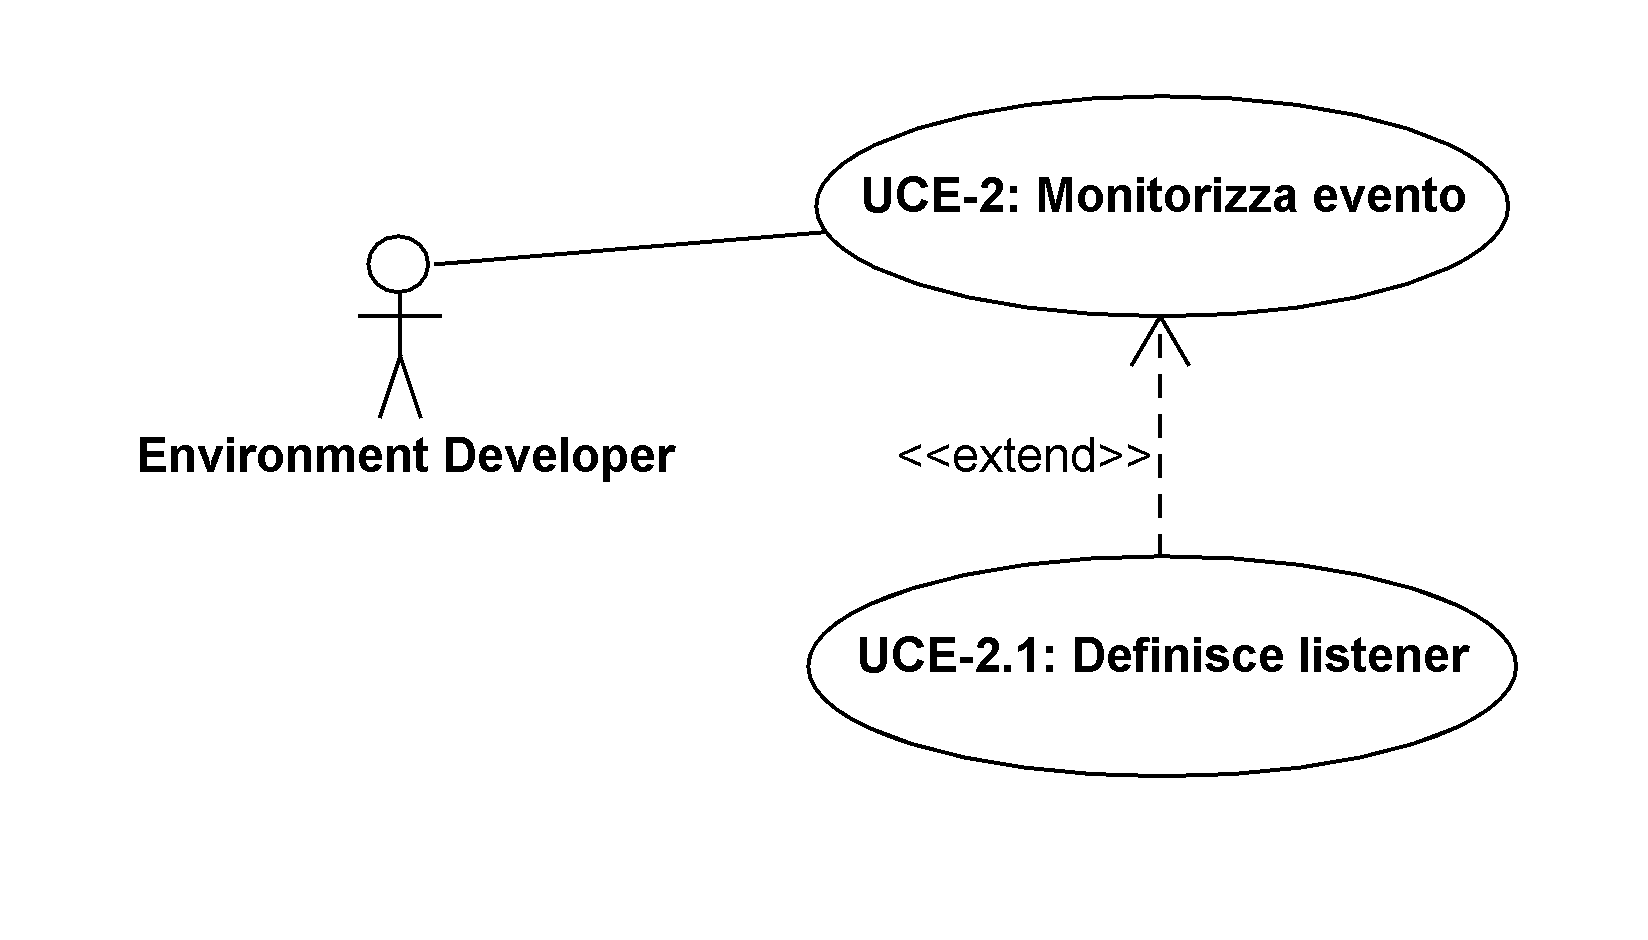
\includegraphics[width=1.1\textwidth]{Immagini/Capitolo2/UseCases/UCE-2.png}
\caption{Diagramma dei casi d'uso UCE-2}\label{fig:uc-uce-2}
\end{figure}


\begin{itemize}
	\item \textbf{Attori:} ED
	\item \textbf{Scopo e descrizione:} l'ED deve essere in grado di specificare un nuovo evento e definire un comportamento da associare al verificarsi dell'evento
	\item \textbf{Pre-condizioni:} il software fornisce meccanismi per la definizione e la notifica di un evento
	\item \textbf{Post-condizioni:} il comportamento specificato dall'ED viene eseguito al verificarsi dell'evento atteso
	\item \textbf{Flusso principale degli eventi:}
		\begin{enumerate}
			\item l'ED specifica un nuovo evento
			\item l'ED specifica un \emph{listener} che realizzi un comportamento al verificarsi di un evento (si guardi il caso d'uso \emph{UCE-2.1})
			\item l'ED avvia il sistema
			\item l'ED avvia un'elaborazione
			\item il verificarsi dell'evento provoca l'esecuzione del comportamento definito
		\end{enumerate}
\end{itemize}


\paragraph{UCE-2.1: Definisce listener}

\begin{itemize}
	\item \textbf{Attori:} ED
	\item \textbf{Scopo e descrizione:} un ED deve essere in grado di specificare un comportamento da eseguire al verificarsi di un evento
	\item \textbf{Pre-condizioni:} il sistema è stato configurato correttamente. Il sistema non è attivo
	\item \textbf{Post-condizioni:} il sistema è attivo e un comportamento è associato all'accadere di un evento
	\item \textbf{Flusso principale degli eventi:}
		\begin{enumerate}
			\item l'ED definisce un comportamento nella forma di un entità \emph{listener}
			\item l'ED registra il \emph{listener} nel sistema
		\end{enumerate}
	
\end{itemize}

